\documentclass{article}

\usepackage[dblblindworkshop]{neurips_2026}
\workshoptitle{AIMO Interpretability Challenge}

\usepackage[utf8]{inputenc}
\usepackage[T1]{fontenc}
\usepackage{hyperref}
\usepackage{url}
\usepackage{booktabs}
\usepackage{amsfonts}
\usepackage{amsmath}
\usepackage{nicefrac}
\usepackage{microtype}
\usepackage{xcolor}
\usepackage{graphicx}

% marks numbers that are still waiting for a leaderboard run; must not remain in the submitted PDF
\newcommand{\pending}{\textcolor{red}{pend.}}

\title{How Long Will It Think?\\Hidden-State Length Probes Predict the Robustness of Reasoning Models}

\author{Anonymous Author(s)}

\begin{document}

\maketitle

\begin{abstract}
The AIMO Interpretability Challenge asks whether a reasoning model's accuracy on a competition math problem survives meaning-preserving perturbations, given only the problem, the model and a few minutes of compute.
We find that the official labels largely measure how reliably the model solves the problem, and that the model's mean reasoning length, relative to its own typical length, is a much sharper measure of this reliability than its solve rate (AUC 0.84 vs.\ 0.63 on the official training cases, measured from full-length traces).
We therefore read the expected reasoning length out of the model's hidden states twice: from the prompt with a linear probe, and from short budgeted rollouts with a \emph{progress probe} applied to the hidden state at the token cap.
Both probes and their per-model fusion are trained on an unlabelled pool of 322 olympiad problems with self-generated traces, so the official labels are never used for fitting.
A capability-aware threshold places the decision boundary among the problems a model reliably solves, which matters most for gpt-oss-120b at low effort: over the whole pool its reasoning length carries no reliability signal.
On the official training cases, used only for evaluation, the predictor reaches AUC 0.80 and balanced accuracy 0.75. On the validation leaderboard it scores 0.62 (Main) and 0.64 (Small), against 0.48 and 0.50 for a constant.
Replacing the hidden-state readout with the best black-box length estimate from the same samples lowers AUC from 0.82 to 0.60 (95\% CI of the gap: 0.04 to 0.41).
\end{abstract}

\section{Introduction}

Reasoning models can solve olympiad problems and still fail on lightly reworded versions of them~\citep{mirzadeh2025gsmsymbolic}.
The AIMO Interpretability Challenge~\citep{stefanik2026aimointerp} turns this into a prediction task.
Given a model $m$ and an unseen problem $x$, decide whether $m$'s accuracy on $x$ survives a battery of perturbations: rephrasing, renaming, change of domain, distractors, typos and expert edits.
Each decision is made in a fresh process with about three minutes of GPU time, far too little to run the perturbation experiment itself.

We build on three observations.
(i)~The labels mostly measure how reliably $m$ solves $x$, and reasoning length relative to $m$'s typical length measures this more sharply than the solve rate (Section~\ref{sec:data}).
(ii)~The expected reasoning length can be read linearly from hidden states: from the prompt and, more accurately, from partial rollouts at a token cap, at no extra cost (Section~\ref{sec:method}).
(iii)~The decision threshold must sit among the problems the model reliably solves, because only those become cases (Sections~\ref{sec:threshold} and~\ref{sec:where}).
Probes, fusion weights and thresholds are learned from an unlabelled problem pool with self-generated traces, so the official training cases remain a held-out evaluation set.
Our contributions are a label-free white-box pipeline that takes about 100\,s per case; a capability-aware threshold, motivated by the finding that gpt-oss-120b at low effort breaks the usual link between reasoning length and reliability; a white-box ablation on identical samples in which the hidden-state readout beats a black-box length estimate (AUC 0.82 vs.\ 0.60); and code, probes and 9k reasoning traces (supplementary material).

\section{Task, data, and the length hypothesis}
\label{sec:data}

\paragraph{Task.}
A case $(m,x)$ is \emph{robust} if the largest drop in $m$'s accuracy, from the original problem to any perturbation family, is at most 0.10. It is \emph{non-robust} if that drop is at least 0.25.
Cases in between are excluded, and so are cases whose original problem $m$ does not answer consistently correctly.
Seven configurations are evaluated.
Four appear in both tracks: Qwen3.5-4B, Skywork-OR1-Math-7B~\citep{he2025skywork}, Olmo-3-7B-Think and DeepSeek-R1-0528-Qwen3-8B~\citep{deepseek2025r1}.
gpt-oss-120b~\citep{openai2025gptoss} at low, medium and high reasoning effort is evaluated on the Main track only.
The 80 labelled official training cases (36 problems, 74\% robust) are the only labels we use, and we use them only for evaluation.
The validation leaderboard (21 Main and 14 Small cases) is balanced per problem and per model. The final test uses unpublished problems.

\paragraph{Unlabelled pool.}
The pool has 322 problems.
Of these, 300 are recent competition problems with public answers from MathArena~\citep{balunovic2025matharena}: AIME 2023--25, HMMT, SMT, BRUMO, CMIMC and APEX. They include 14 of the 36 official training problems.
The other 22 training problems have no public answer, so we use the majority answer of finished traces as the reference.
For every configuration we sampled traces with vLLM~\citep{kwon2023vllm}, using the organisers' sampling settings (temperature 1, top-$k$ 40, top-$p$ 0.95) and a 32k-token cap.
Qwen and Skywork have 4 traces per problem and gpt-oss has 6. Olmo has 3--4 traces on a 108-problem subset, and DeepSeek has 2 on a 144-problem subset.
In total this is 9{,}056 traces and 114M tokens, about \$80 of rented GPU time.
We stored the hidden states of every prompt and of every trace prefix at the deployed token caps (Section~\ref{sec:method}).

\paragraph{The length hypothesis.}
Our traces cover 79 of the 80 training cases.
For these, the \emph{relative length} is the mean log trace length of $m$ on $x$ minus the median over $m$'s pool.
This oracle quantity separates the labels with AUC 0.84, and the rule ``shorter than the median'' is 80\% accurate.
The solve rate reaches only AUC 0.63 because it saturates.
78\% of cases are solved in every trace, including 12 of the 20 non-robust ones.
A robust case is one the model solves \emph{with margin}, and a short trace is evidence of margin.
The rest of this paper estimates relative length without generating full traces.

\section{Method}
\label{sec:method}

\begin{figure}[t]
  \centering
  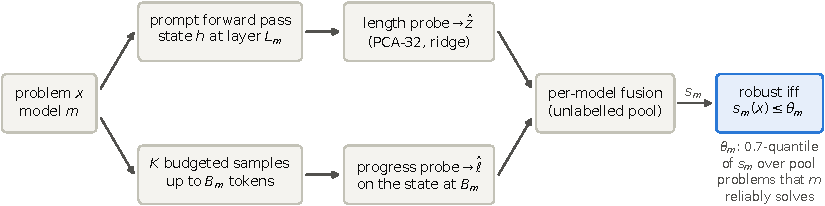
\includegraphics[width=\linewidth]{figures/fig_pipeline.pdf}
  \caption{Per-case pipeline. Both probes estimate the mean log reasoning length of model $m$ on problem $x$. Probes, fusion weights and the threshold $\theta_m$ are fitted on an unlabelled problem pool; the official robustness labels are not used.}
  \label{fig:pipeline}
\end{figure}

\paragraph{Prompt probe.}
Figure~\ref{fig:pipeline} shows the per-case pipeline.
We run one forward pass over the chat-formatted prompt, using the organisers' solve prompt and, for gpt-oss, the requested reasoning effort.
We take the residual stream at layer $L_m$, either at the last token or averaged over the problem span.
We standardise it, project it onto 32 principal components and fit a ridge regression ($\alpha = 10$).
The target is the problem's mean log trace length $\bar\ell_m(x)$; a trace cut at 32k tokens counts at the cap.
Layer and pooling are chosen per configuration by five-fold cross-validation on the pool, with near-duplicate problem templates kept in the same fold.
The result is $\hat z_m(x)$.

\paragraph{Progress probe.}
At test time we sample $K$ traces in parallel up to a token cap $B_m$. $B_m$ is sized so that sampling ends within the time budget: 1.5k--4k tokens, with $K$ = 16--64 (Table~\ref{tab:probes}).
A forward hook keeps the layer-$L'_m$ state of the last generated token of every trace. This is free, because that forward pass runs anyway.
For traces still running at $B_m$, a second probe with the same recipe maps this state to the problem's mean log length.
Finished traces contribute their observed log length instead.
The estimate $\hat\ell_m(x)$ averages over the $K$ traces.
We train this probe on states recomputed offline for every pool trace truncated at exactly $B_m$ tokens, so training and deployment see the same distribution.

\paragraph{Label-free fusion.}
For each configuration, $s_m(x) = a_0 + a_1 \hat z_m(x) + a_2 \hat\ell_m(x) - c_m$.
The weights $a$ are fitted by least squares to $\bar\ell_m$ on out-of-fold pool predictions, and $c_m$ is the pool median of the fused value.
Because the validation set is balanced per model, scores are compared only within a model.

\paragraph{Capability-aware threshold.}
\label{sec:threshold}
A case is predicted robust if $s_m(x) \le \theta_m$.
Centring at the pool median ($\theta_m = 0$) assumes that the boundary between robust and non-robust cases lies at the median pool problem.
A case exists only if $m$ solves $x$ consistently, though, so the boundary lies inside $\mathcal{B}_m$, the set of pool problems that $m$ reliably solves.
A problem is in $\mathcal{B}_m$ if at least one trace finished and every finished trace is correct.
Traces cut at 32k count as unknown, because labels use a 100k budget.
We set $\theta_m$ to the $\rho$-quantile of $s_m$ over $\mathcal{B}_m$, with $\rho = 0.7$.
This is slightly below the natural robust rate among consistently solved training cases (0.74), to hedge towards balanced test populations.
No parameter is fitted to the official labels; $\rho$ is the only quantity they inform.

\paragraph{Runtime.}
Each case runs in a fresh process: model load takes 2--6\,s, the prompt pass under 4\,s and sampling about 90\,s.
On the validation server the full pipeline took 88--104\,s per case, with no failures.
If sampling or the hook fails, the case falls back to $\hat z_m$ with its own capability-aware threshold.

\section{Results}
\label{sec:results}

\begin{table}[t]
  \caption{Probe quality and deployed settings per configuration (pool: 322 problems; Olmo 108, DeepSeek 144). $\rho$: Spearman correlation between out-of-fold predictions and the true mean log trace length on the pool. AUC: threshold-free AUC of $-s_m$ on the official training cases. $L_m$: prompt-probe layer; $B_m$, $K$: token cap and number of traces at test time.}
  \label{tab:probes}
  \centering
  \resizebox{\linewidth}{!}{%
  \begin{tabular}{lrrrrrrcrr}
    \toprule
    Configuration & $L_m$ & $B_m$ & $K$ & $\rho_{\text{prompt}}$ & $\rho_{\text{progress}}$ & $\rho_{\text{fused}}$ & train cases (robust) & AUC & $\theta_m$ \\
    \midrule
    Qwen3.5-4B        & 32 & 3072 & 32 & 0.69 & 0.54 & 0.72 & 12 (8)  & 0.88 & $-0.04$ \\
    Skywork-OR1-7B    & 21 & 4096 & 64 & 0.52 & 0.48 & 0.56 & 12 (9)  & 0.78 & $-0.05$ \\
    Olmo-3-7B-Think   & 16 & 2560 & 16 & 0.53 & 0.26 & 0.55 & 9 (7)   & 0.64 & $-0.03$ \\
    DeepSeek-R1-8B    & 27 & 3072 & 32 & 0.44 & 0.36 & 0.50 & 10 (7)  & 0.81 & $-0.04$ \\
    gpt-oss low       & 24 & 1536 & 40 & 0.39 & 0.99 & 0.98 & 7 (5)   & 0.80 & $+0.17$ \\
    gpt-oss medium    & 24 & 1536 & 40 & 0.46 & 0.74 & 0.74 & 15 (10) & 1.00 & $-0.01$ \\
    gpt-oss high      & 18 & 1536 & 40 & 0.63 & 0.70 & 0.74 & 15 (13) & 0.73 & $+0.16$ \\
    \bottomrule
  \end{tabular}}
\end{table}

\paragraph{Probe quality.}
Table~\ref{tab:probes} reports probe quality per configuration.
From the prompt alone, the probe predicts the model's own mean log reasoning length with Spearman correlation 0.39--0.69.
The progress probe matters most where many traces finish before the cap.
For gpt-oss low, 50--75\% of traces finish within 1.5k tokens, so $\hat\ell$ is close to the observed length ($\rho = 0.99$).
For long-reasoning models nearly all traces are still running at the cap, and the state at the cap carries most of the signal.
Fusion reaches 0.50--0.98.
Olmo and DeepSeek have the least training data (108 and 144 problems, 2--4 traces each) and the weakest probes.

\begin{table}[t]
  \caption{Robustness prediction on the official training cases (held out: no component is fitted to them) and on the validation leaderboard. AUC is threshold-free; accuracy and balanced accuracy use each method's deployed threshold. The 61-case subset is where we recorded samples with the deployed sampler (Qwen, Skywork, gpt-oss), so every method sees the same cases. The black-box row uses the same samples as the white-box rows but only their lengths and finish flags (censored log-normal estimate of the mean log length).}
  \label{tab:ablation}
  \centering
  \resizebox{\linewidth}{!}{%
  \begin{tabular}{llccccccc}
    \toprule
    & & \multicolumn{3}{c}{train, all 80} & \multicolumn{2}{c}{train, 61 with samples} & \multicolumn{2}{c}{validation acc.} \\
    \cmidrule(lr){3-5}\cmidrule(lr){6-7}\cmidrule(lr){8-9}
    Method & hidden states & AUC & acc & bal.\ acc & AUC & bal.\ acc & Main & Small \\
    \midrule
    constant ``robust''                & --  & --   & 0.738 & 0.500 & --   & 0.500 & 0.476 & 0.500 \\
    black-box length, same samples     & no  & --   & --    & --    & 0.603 & 0.578 & 0.619 & 0.571 \\
    prompt probe $\hat z$, $\theta^z_m$ & yes & 0.768 & 0.700 & 0.689 & 0.790 & 0.719 & 0.667 & 0.571 \\
    fused $s$, train-fitted threshold  & yes & 0.804 & 0.688 & 0.711 & 0.818 & --    & 0.571 & -- \\
    fused $s$, $\theta_m = 0$          & yes & 0.804 & 0.762 & 0.716 & 0.818 & 0.764 & 0.619 & 0.643 \\
    \textbf{fused $s$, capability $\theta_m$ (final)} & yes & \textbf{0.804} & \textbf{0.787} & \textbf{0.749} & \textbf{0.818} & \textbf{0.786} & \textbf{0.619} & \textbf{0.643} \\
    \bottomrule
  \end{tabular}}
\end{table}

\paragraph{Robustness prediction and the white-box ablation.}
Table~\ref{tab:ablation} compares the methods on the training cases and the validation leaderboard.
Because nothing is fitted to the training cases, they act as a held-out set of 80 cases.
On the 61 cases where we recorded samples with the deployed sampler, the black-box row uses those same samples but only their lengths and finish flags, the information a self-consistency-style method~\citep{wang2023selfconsistency} has at this budget.
Its estimate of the mean log length reaches AUC 0.60; reading the hidden states of the same samples raises this to 0.82 (95\% CI of the difference, bootstrap over problem templates: 0.04 to 0.41), and balanced accuracy from 0.58 to 0.79.
At a budget of a few thousand tokens almost no trace of a long-reasoning model finishes, but the hidden state at the cap still reveals how far the model is from an answer.
Within the white-box family, adding the progress probe to the prompt probe raises AUC from 0.77 to 0.80, a gap within noise (CI $-0.07$ to $0.12$).
On the validation leaderboard, our first submission used a threshold fitted to the training cases and predicted only 3 of 21 cases robust (accuracy 0.571): the training cases are easier than the validation problems (median $s = -0.20$ vs.\ $0.00$), which motivated the thresholds of Section~\ref{sec:threshold}.
The final predictor scores 0.619 on Main (13/21) and 0.643 on Small (9/14), against 0.476 and 0.500 for a constant.
The 35 validation cases cannot separate it from the black-box ablation (22 vs.\ 21 correct) or from the prompt probe alone (also 22 correct). When no trace finishes within the budget, which is the case for every configuration except gpt-oss low, the black-box estimate falls back to the model's prior and acts as a per-model constant, which scores about one half on a set balanced per model.

\begin{figure}[t]
  \centering
  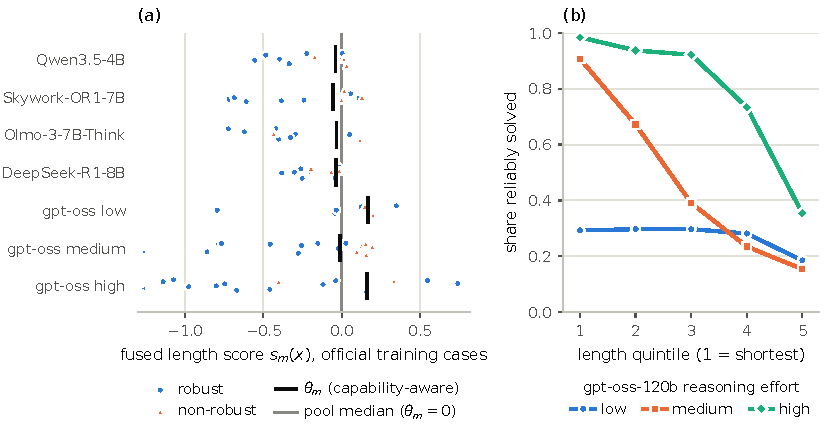
\includegraphics[width=\linewidth]{figures/fig_main.pdf}
  \caption{(a) Fused score $s_m(x)$ of the official training cases (not used for fitting) with the pool-median threshold (grey) and the capability-aware threshold $\theta_m$ (black). Two robust cases at $s < -1.3$ are drawn at the left edge. (b) Pool problems: share reliably solved (every finished trace correct) by quintile of the model's own mean reasoning length. At low effort, length carries no reliability signal over the whole pool.}
  \label{fig:main}
\end{figure}

\paragraph{Where the threshold belongs.}
\label{sec:where}
Figure~\ref{fig:main}b shows why the pool median is a poor boundary for some models.
For gpt-oss at medium and high effort, a short trace means the problem is reliably solved.
At low effort, the share of reliably solved problems is flat at about 0.30 across the first four length quintiles, because low-effort reasoning stays short on problems the model fails.
Over the whole pool, its mean length is even weakly anti-correlated with its solve rate (Spearman $-0.20$), whereas the other configurations range from $+0.53$ to $+0.97$.
Restricted to $\mathcal{B}_m$, where cases come from, the ordering returns for every configuration.
There, $s_m$ correlates positively with the other models' failure rate on the same problem: $+0.22$ for gpt-oss low and $+0.21$ to $+0.68$ elsewhere.
The capability-aware threshold therefore moves $\theta_m$ to $+0.17$ for gpt-oss low and $+0.16$ for high, and keeps it within $0.06$ of zero for the other configurations (Figure~\ref{fig:main}a).
On the training cases it raises balanced accuracy from 0.716 to 0.749 and accuracy from 0.762 to 0.787. These are only 2--3 cases, so the main argument for it is the mechanism, not the gain.

\section{Discussion}
Reasoning models appear to carry an internal estimate of how much computation a problem will need, much as language models encode whether they know an answer~\citep{kadavath2022know,azaria2023internal}.
A linear probe~\citep{alain2016probes,belinkov2022probing} can read this estimate before generation starts and read it better a few thousand tokens in.
The robustness labels track the margin by which a model solves a problem. Expected reasoning length is a good proxy for that margin, and it can be estimated without labels, which suits a task with only 80 labelled cases.
The method has one free parameter, $\rho$, that is set with knowledge of the training labels.
It runs in about 100\,s per case and degrades gracefully: if sampling fails, the prompt probe alone still gives AUC 0.77.

\section*{Limitations}
Only 80 labelled cases exist, so per-model AUCs rest on 7--15 cases and the confidence intervals above are wide.
The validation leaderboard has 21 or 14 cases, so a single score has a standard error of about 0.11.
Our traces are capped at 32k tokens while labels use 100k. This biases the target for long-reasoning models (Qwen and DeepSeek have a truncated trace on 71--77\% of pool problems), and it is why traces cut at the cap count as unknown in $\mathcal{B}_m$.
DeepSeek and Olmo have the least data.
The test may label some problems with an expert ``no solution'' family, which train-main-v2 does not include. A model that never answers ``no solution'' would be non-robust on such a problem whatever its difficulty, and our length signal cannot see this.
Finally, the test distribution is not guaranteed to be balanced. The threshold choice ($\rho = 0.7$) hedges between balanced and natural label rates rather than optimising for either.

\section*{AI Use Statement}
In this work, we used generative AI tools (Anthropic's Claude, operating as a coding agent in Claude Code) for ideation and literature search, for implementing all code and data pipelines, for running and analysing experiments, for creating the figures, and for drafting and editing this report.
The authors set the goals and the compute budget, made all leaderboard submissions, and selected the final submissions.
We did not use generative AI tools to produce any data labels: the reference answers come from the original competitions or, for 22 training problems, from the majority answer of the evaluated models' own traces, as described in Section~\ref{sec:data}.
We have reviewed all AI-assisted work and take responsibility for the final content of this paper, including AI-assisted text, claims, code and other artifacts.

\bibliographystyle{plainnat}
\bibliography{refs}

\appendix

\section{Reproducibility}
\label{app:repro}
The supplementary archive contains the submission bundle, the training code, the problem pool, all 9{,}056 traces (answers, lengths, finish flags) and the trained probes.
The hidden-state dumps (1.2\,GB) exceed the archive limit; we will release them after the review period, and they can be regenerated, up to sampling randomness, with the included generation and extraction scripts.
On a laptop CPU, the full training pipeline below reproduces the submitted probe artifacts bit for bit:
{\footnotesize
\begin{verbatim}
python experiments/train_probe.py --gen G/gen --hidden G/hidden --art A/probe --report R
python experiments/train_progress.py --gen G/gen --progress G/progress \
       --art A/probe --out A/prog --report R
python experiments/fuse.py --report R --art A/prog --out A/fused
python experiments/capability_threshold.py --report R --art A/fused --rho 0.7 --out A/final
python experiments/build_submission.py --art A/final --name final
\end{verbatim}
}
Data generation (GPU) uses \texttt{cloud/gen\_solve.py} (vLLM, organisers' sampling, 32k cap), \texttt{cloud/extract\_hidden.py} (prompt states) and \texttt{cloud/extract\_progress.py} (states of trace prefixes truncated at $B_m$).
At test time, the bundle needs only the evaluation image (PyTorch, Transformers 5.13); vLLM is used only for data generation.

\section{Engineering notes}
\begin{itemize}
  \item With Transformers 5.13 and 5.19, \texttt{AutoTokenizer} for DeepSeek-R1-0528-Qwen3-8B silently drops all spaces on encode and decode. We select the tokenizer by a round-trip check and pass token ids to vLLM.
  \item For gpt-oss-120b, native MXFP4 inference in Transformers requires the \texttt{kernels} package in [0.15.2, 0.16). Newer versions silently dequantise to bf16 and run out of memory. In vLLM, a single 96\,GB GPU ran out of memory during weight repacking; tensor parallelism 2 with the Triton attention backend worked.
  \item Final-layer states of gpt-oss at medium and high effort overflow fp16, so non-finite layers are skipped when selecting the progress layer.
  \item Qwen3.5-4B (hybrid linear attention) decodes at about 27\,ms per step at batch 32 in Transformers, because linear attention falls back to a PyTorch implementation. Olmo-3-7B-Think is attention-bound (32 KV heads). These two drove the per-model choice of $K$ and $B_m$.
\end{itemize}
\end{document}
